\chapter{طرائق المعايرة ومنحنياتها}\label{ch:b1:titration-methods}

تتسلّم صيدلانية دفعة من أقراص الفيتامين C مكتوبًا عليها
\qty{500}{mg}، وعليها أن تشهد، قبل بيعها، أن كل قرص يحوي
ما تقوله اللصاقة. ولن تزن الفيتامين مباشرة: فهو
ممزوج بمواد رابطة ومالئة. بل ستعايره --- أي تجعله يتفاعل مع
كاشف معلوم التركيز، وتقيس الحجم اللازم، وتحسب
الكمية. أي تفاعل، وكيف تُرى نهايته، وما مدى الثقة بالنتيجة:
تلك أسئلة هذا الفصل، الذي ينقل توازنات
الفصول الخمسة السابقة إلى طاولة المختبر.

\begin{recall}
عاير المجلد المدرسي (الصفان الحادي عشر والثاني عشر) الأحماض بالقواعد بتغير
اللون، وتتبّع المعايرات بمقياس pH وبمقياس
الموصلية، واستعمل علاقة \omterm{def:b1:titration-methods:titration}{التكافؤ} $C_AV_A = C_BV_B$. وطريقة
\omterm{def:b1:predominant-reaction:predominant-reaction}{التفاعل الغالب} في \cref{ch:b1:predominant-reaction}؛ وتوازنات
الترسيب والتعقيد والأكسدة والاختزال في
\cref{ch:b1:precipitation,ch:b1:complexation,ch:b1:nernst}.
\end{recall}

\begin{omfigure}
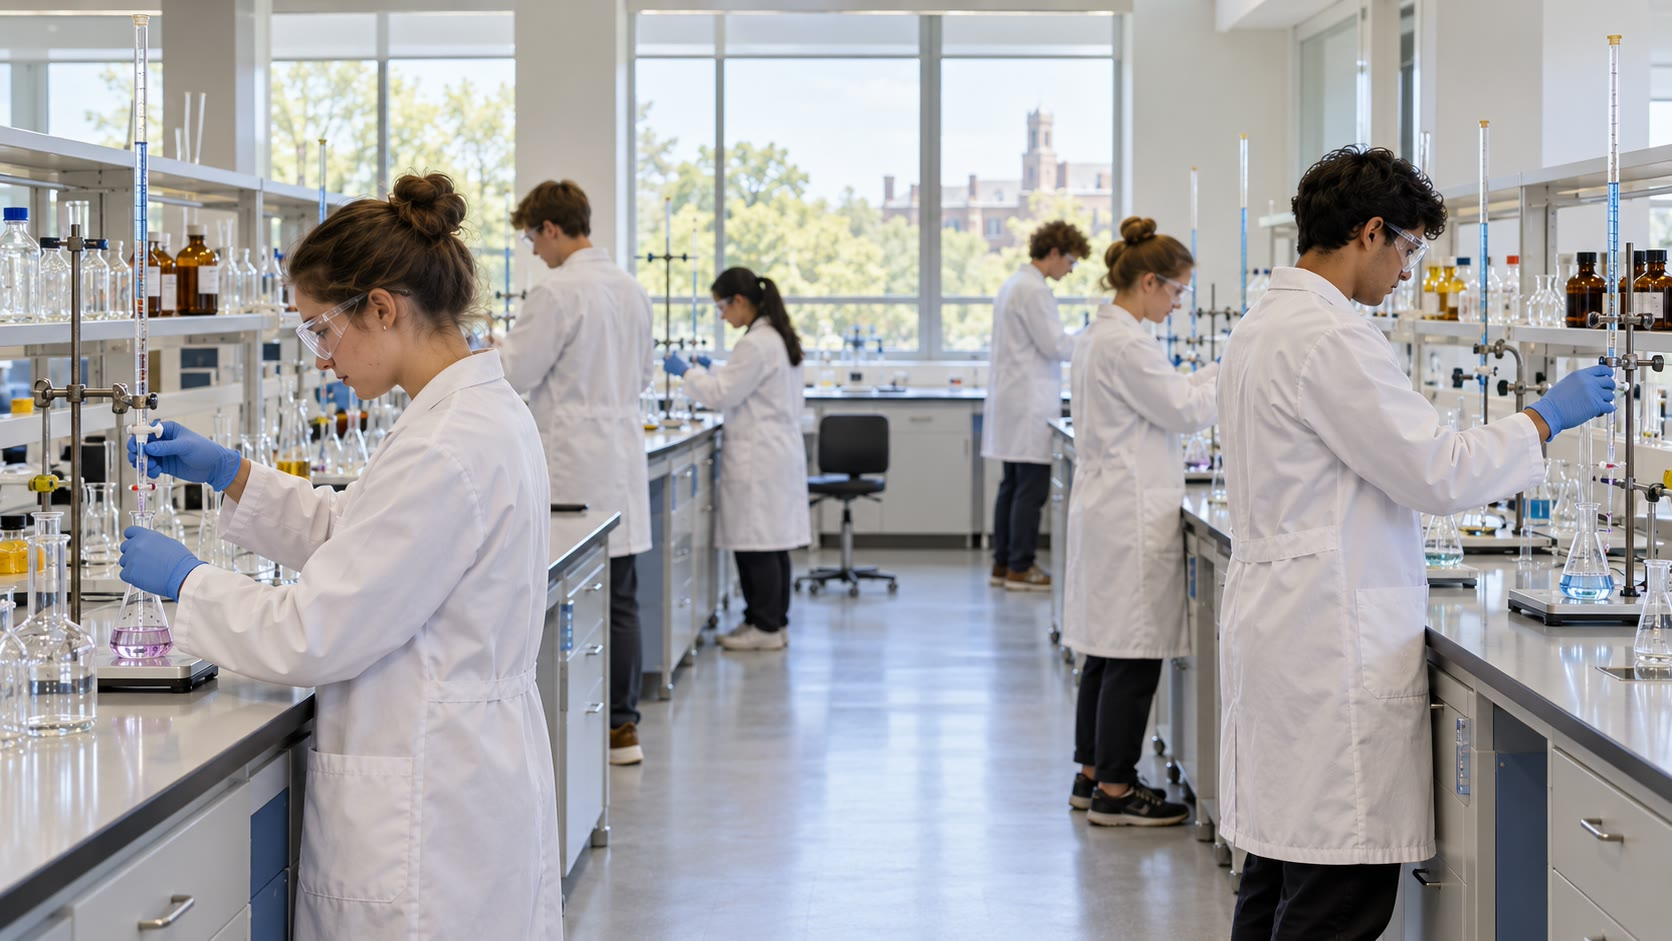
\includegraphics[width=0.66\linewidth]{images/book2/ai/b1-15-teaching-lab.jpg}

{\small مختبر تعليمي: سحاحة، ودورق مخروطي على مخلاط
مغناطيسي، وقفازات ونظارات واقية. \omterm{def:b1:titration-methods:titration}{والمعايرة} أشيع قياسات المقادير
في الكيمياء.}
\end{omfigure}

\section{المعايرة والتكافؤ}

\begin{definition}[المعايرة، التكافؤ]\label{def:b1:titration-methods:titration}
\emph{المعايرة}\index{معايرة} تعيّن كمية نوع كيميائي،
هو \emph{المادة المعايَرة}\index{مادة معايَرة}، بتفاعل مع كاشف معلوم
التركيز، هو \emph{المحلول المعايِر}\index{محلول معايِر}، يضاف تدريجيًا.
ويجب أن يكون التفاعل وحيدًا، \omterm{def:b1:extent-q-and-k:quantitative}{وكمّيًا} ($K$ كبير) وسريعًا. ويُبلغ
\emph{التكافؤ}\index{تكافؤ} حين يكون المحلول المعايِر والمادة المعايَرة
قد جُمعا بالنسب الستوكيومترية
للتفاعل؛ ويكون الحجم المضاف عندئذ حجم التكافؤ، والنقطة
من منحنى المعايرة عند ذلك الحجم هي \emph{نقطة
التكافؤ}\index{نقطة التكافؤ}. أما الحجم الذي يتوقف عنده المجرِّب،
حين يرى تغير لون أو انكسارًا في منحنى، فهو \emph{نقطة
النهاية}\index{نقطة النهاية}؛ والطريقة الجيدة تجعلها تنطبق على
التكافؤ.
\end{definition}

\begin{proposition}[علاقة التكافؤ]\label{prop:b1:titration-methods:equivalence}
من أجل تفاعل \omterm{def:b1:titration-methods:titration}{معايرة} $a\,\mathrm{A} + b\,\mathrm{B} \to \cdots$، مع
\omterm{def:b1:titration-methods:titration}{المادة المعايَرة} A (بكمية $n_A$ مول) \omterm{def:b1:titration-methods:titration}{والمحلول المعايِر} B بتركيز $C_B$، يحقق
حجم \omterm{def:b1:titration-methods:titration}{التكافؤ}
\[
  \frac{n_A}{a} = \frac{C_B V_{\mathrm{eq}}}{b} .
\]
\end{proposition}

\begin{proof}
ليكن $x$ التقدم بعد إضافة الحجم $V$ من \omterm{def:b1:titration-methods:titration}{المحلول المعايِر}. قبل \omterm{def:b1:titration-methods:titration}{التكافؤ} يكون B
هو المحدِّد، ولأن التفاعل كمّي يكون $x = C_BV/b$؛ وبعده
يكون A هو المحدِّد و$x = n_A/a$. \omterm{def:b1:titration-methods:titration}{والتكافؤ} هو الحجم الذي يُستهلك فيه الاثنان
معًا، $n_A - ax = 0$ و$C_BV - bx = 0$: وبحذف $x$
نحصل على العلاقة.
\end{proof}

\section{المعايرات المباشرة وغير المباشرة}

\begin{definition}[أنواع المعايرة]\label{def:b1:titration-methods:kinds}
في \emph{المعايرة المباشرة}\index{معايرة مباشرة} يتفاعل \omterm{def:b1:titration-methods:titration}{المحلول المعايِر}
مع \omterm{def:b1:titration-methods:titration}{المادة المعايَرة} نفسها. وفي \emph{المعايرة العكسية}\index{معايرة عكسية}
يضاف إلى \omterm{def:b1:titration-methods:titration}{المادة المعايَرة} فائض معلوم من كاشف، ثم يُعاير الفائض الباقي.
وحين يحوي محلول عدة مواد معايَرة تتفاعل
بالتتابع مع \omterm{def:b1:titration-methods:titration}{المحلول المعايِر}، تقاس \emph{بمعايرات
متتالية}\index{معايرات متتالية}، تكافؤًا بعد \omterm{def:b1:titration-methods:titration}{تكافؤ}؛
وحين تتفاعل معًا وتعطي تكافؤًا واحدًا، تقاس \emph{بمعايرة
متزامنة}\index{معايرة متزامنة}، لا تعطي
إلا مجموعها.
\end{definition}

\begin{method}[المعايرة العكسية]\label{met:b1:titration-methods:back-titration}
استعملها حين يكون التفاعل المباشر بطيئًا، أو تكون \omterm{def:b1:titration-methods:titration}{المادة المعايَرة} غير مستقرة أو
متطايرة، أو حين لا يلائم أي \omterm{def:b1:titration-methods:indicator}{كاشف ملوّن} التفاعل المباشر.
\begin{enumerate}
  \item أضف كمية معلومة $n_R$ من الكاشف R، بفائض، ودعه يتفاعل
        تفاعلًا تامًا مع \omterm{def:b1:titration-methods:titration}{المادة المعايَرة} \babelsublr{A ($\alpha\,\mathrm{A} + \rho\,\mathrm{R}$)}.
  \item عاير فائض R \omterm{def:b1:titration-methods:titration}{بمحلول معايِر} \babelsublr{T ($\rho'\,\mathrm{R} +
        \tau\,\mathrm{T}$)} حتى حجم \omterm{def:b1:titration-methods:titration}{التكافؤ} $V_T$.
  \item احسب $n_{R,\text{فائض}} = \frac{\rho'}{\tau}C_TV_T$، ثم
        $n_A = \frac{\alpha}{\rho}(n_R - n_{R,\text{فائض}})$.
\end{enumerate}
\end{method}

تعاير مسألة نهاية الأسبوع الفيتامين C بهذه الطريقة: يختزل حمض الأسكوربيك
فائضًا من اليود، ثم يُعاير اليود الباقي بالثيوكبريتات.

\section{المعايرات بقياس pH والكواشف الملوّنة}

\begin{omfigure}
\begin{tikzpicture}[font=\small]
  \pic at (0,0) {stirrer};
  \pic at (0,0.18) {beaker={0.55}{omDef!14}};
  \pic at (0.2,2.45) {burette={0.75}{white}};
  \pic at (-0.45,0.45) {probe};
  \pic (m) at (-2.6,3.2) {meter={pH}};
  \draw[thick] (-0.45,3.45) to[out=90, in=0] (m-b);
  \node[anchor=west] at (0.65,6.2) {\foreignlanguage{arabic}{السحاحة: \babelsublr{NaOH}، \qty{0.100}{mol/L}}};
  \node[anchor=west] at (1.0,1.0) {\foreignlanguage{arabic}{الحمض، $V_0 = \qty{10.0}{mL}$، مخففًا}};
  \draw[<-, omProp, thick] (1.2,-0.25) -- (1.8,-0.25) node[anchor=west, text=black] {مخلاط مغناطيسي};
  \draw[<-, omProp, thick] (-0.62,2.4) -- (-1.5,2.0) node[anchor=east, text=black] {قطب مركّب};
\end{tikzpicture}

{\small \omterm{def:b1:titration-methods:titration}{معايرة} بقياس pH. يقيس القطب الزجاجي المركّب
pH بعد كل إضافة من السحاحة؛ ويمزج المخلاط المحلول.
ويُعايَر القطب مسبقًا بمحلولين منظمين.}
\end{omfigure}

\begin{omfigure}
\begin{tikzpicture}
\begin{axis}[name=s,
  width=0.5\linewidth, height=5.6cm, xmin=0, xmax=20, ymin=0, ymax=14,
  axis x line=bottom, axis y line=left, xlabel={\babelsublr{$V$ (mL)}}, ylabel={\babelsublr{pH}},
  xtick={0,5,10,15,20}, ytick={0,2,4,6,8,10,12,14},
  tick label style={font=\small}, label style={font=\small}]
\addplot[omDef, very thick] table[x=V, y=pH] {figdata/out/bachelor-1-titration-curves-strong.dat};
\addplot[omProp, thick] table[x=V, y=pH] {figdata/out/bachelor-1-titration-curves-weak.dat};
\node[font=\scriptsize, omDef, anchor=south west] at (axis cs:6,0.2) {\ce{HCl}};
\node[font=\scriptsize, omProp, anchor=west] at (axis cs:0.4,6.4) {\ce{CH3COOH}};
\draw[dotted] (axis cs:5,0) -- (axis cs:5,4.76) -- (axis cs:0,4.76);
\node[font=\scriptsize, anchor=north] at (axis cs:2.5,4.7) {$\mathrm{p}K_a$};
\end{axis}
\begin{axis}[at={(s.east)}, anchor=west, xshift=1.2cm,
  width=0.5\linewidth, height=5.6cm, xmin=0, xmax=20, ymin=0, ymax=14,
  axis x line=bottom, axis y line=left, xlabel={\babelsublr{$V$ (mL)}}, ylabel={\babelsublr{pH}},
  xtick={0,5,10,15,20}, ytick={0,2,4,6,8,10,12,14},
  tick label style={font=\small}, label style={font=\small}]
\addplot[omMeth, very thick] table[x=V, y=pH] {figdata/out/bachelor-1-titration-curves-mixture.dat};
\node[font=\scriptsize, anchor=west, align=left] at (axis cs:10.8,6.0) {\ce{HCl} + \ce{CH3COOH}\\ تكافؤان};
\end{axis}
\end{tikzpicture}

{\small يسارًا: \qty{10.0}{mL} من حمض الكلوريدريك ومن حمض الإيثانويك،
كلاهما بتركيز \qty{0.100}{mol/L}، معايَرين بهيدروكسيد الصوديوم بتركيز
\qty{0.100}{mol/L}. \omterm{def:b1:predominant-reaction:strong-acid}{للحمض الضعيف} منطقة تنظيم فيها \babelsublr{pH $=
\mathrm{p}K_a$} عند نصف \omterm{def:b1:titration-methods:titration}{التكافؤ}، \omterm{def:b1:titration-methods:titration}{ونقطة تكافؤ} عند pH 8.73.
يمينًا: خليط، \qty{0.050}{mol/L} من كل حمض: يُعاير \omterm{def:b1:predominant-reaction:strong-acid}{الحمض القوي}
أولًا (\omterm{def:b1:titration-methods:titration}{التكافؤ} عند \qty{5}{mL})، ثم الضعيف
(\qty{10}{mL}).}
\end{omfigure}

\begin{proposition}[نصف تكافؤ حمض ضعيف]\label{prop:b1:titration-methods:half-equivalence}
حين يُعاير \omterm{def:b1:predominant-reaction:strong-acid}{حمض ضعيف} HA \omterm{def:b1:predominant-reaction:strong-acid}{بقاعدة قوية}، يكون عند نصف \omterm{def:b1:titration-methods:titration}{التكافؤ}
$\mathrm{pH} = \mathrm{p}K_a$، بشرط ألا يكون الحمض قويًا جدًا
ولا مخففًا جدًا ($\mathrm{p}K_a$ بين 4 و10 تقريبًا عند
\qty{0.1}{mol/L}).
\end{proposition}

\begin{proof}
عند نصف \omterm{def:b1:titration-methods:titration}{التكافؤ} يكون التفاعل الكمّي \ce{HA + OH- -> A- + H2O}
قد حوّل نصف HA: $[\mathrm{HA}] = [\mathrm{A^-}]$،
وتعطي علاقة هندرسون $\mathrm{pH} = \mathrm{p}K_a$. ويضمن الشرط
أن تفاعل HA مع الماء وتفاعل $\mathrm{A^-}$
مع الماء لا يغيّران هاتين الكميتين تغييرًا ملحوظًا.
\end{proof}

\begin{proposition}[pH عند تكافؤ حمض ضعيف]\label{prop:b1:titration-methods:ph-at-equivalence}
عند \omterm{def:b1:titration-methods:titration}{تكافؤ} \omterm{def:b1:predominant-reaction:strong-acid}{حمض ضعيف} ($\mathrm{p}K_a$) \omterm{def:b1:predominant-reaction:strong-acid}{بقاعدة قوية}، يكون
المحلول محلول القاعدة المرافقة بتركيز $C'$ (بعد التخفيف)، و
\[
  \mathrm{pH} = \tfrac12(\mathrm{p}K_e + \mathrm{p}K_a + \log C') .
\]
\end{proposition}

\begin{proof}
\omterm{def:b1:predominant-reaction:predominant-reaction}{للتفاعل الغالب} للقاعدة مع الماء،
\ce{A- + H2O <=> HA + OH-}، الثابت $K = K_e/K_a$؛ ومع تحوّل قليل
من القاعدة، $[\ce{OH-}] = \sqrt{KC'}$ (\cref{prop:b1:predominant-reaction:ph-formulas})،
ومنه النتيجة. ومن أجل حمض الإيثانويك، $C' = \qty{0.050}{mol/L}$:
$\frac12(14.00 + 4.76 - 1.30) = 8.73$.
\end{proof}

\begin{proposition}[المعايرات المتتالية]\label{prop:b1:titration-methods:successive}
يعطي حمضان يُعايَران بالقاعدة نفسها تكافؤين منفصلين، كل منهما بدقة
أفضل من \qty{1}{\percent}، إذا اختلفت قيمتا $\mathrm{p}K_a$ لهما بمقدار 4 على الأقل.
\end{proposition}

\begin{proof}
عند \omterm{def:b1:titration-methods:titration}{التكافؤ} الأول، يكون لتفاعل القاعدة $\mathrm{A_1^-}$ مع
الحمض الثاني $\mathrm{HA_2}$، $\mathrm{A_1^-} + \mathrm{HA_2}
\rightleftharpoons \mathrm{HA_1} + \mathrm{A_2^-}$، الثابت $K = 10^{\mathrm{p}K_1 - \mathrm{p}K_2}$.
وانطلاقًا من كميتين متساويتين، يحقق الكسر $x$ من الحمض الثاني الذي
عُوير أصلًا $x^2/(1 - x)^2 = K$؛ ومن أجل $x \leqslant 0.01$، يكون $K
\leqslant 10^{-4}$، أي $\mathrm{p}K_2 - \mathrm{p}K_1 \geqslant 4$.
\end{proof}

يعطي حمض الفوسفوريك (2.15، 7.21، 12.34) تكافؤين واضحين؛ أما
الثالث فيضيع في ماء القاعدة. وحمض الإيثانويك الممزوج
بحمض الكلوريدريك (يمين الشكل) يُعاير بعده، إذ يكون \omterm{def:b1:predominant-reaction:strong-acid}{الحمض
القوي} في الواقع ذا $\mathrm{p}K_a$ أدنى من 0.

\begin{method}[تعيين التكافؤ على منحنى]\label{met:b1:titration-methods:derivative}
\begin{enumerate}
  \item المشتقة: احسب $\Delta\mathrm{pH}/\Delta V$ بين
        النقاط المتتالية؛ فيقع \omterm{def:b1:titration-methods:titration}{التكافؤ} عند قيمتها العظمى.
  \item المماسات: ارسم مماسين متوازيين للمنحنى على جانبي
        القفزة، والموازي الواقع على بعد متساوٍ منهما؛ فهو يقطع
        المنحنى عند \omterm{def:b1:titration-methods:titration}{نقطة التكافؤ}.
\end{enumerate}
\end{method}

\begin{method}[المماسات بالحساب]\label{met:b1:titration-methods:tangents}
في منحنى مسجّل بالحاسوب، طابق نقاط كل جانب من
القفزة بدالة ملساء وخذ نقطة الانعطاف؛ وفي
القفزة المتناظرة (\omterm{def:b1:predominant-reaction:strong-acid}{حمض قوي}، \omterm{def:b1:predominant-reaction:strong-acid}{قاعدة قوية}) يكون منتصف القفزة عند pH
7 هو \omterm{def:b1:titration-methods:titration}{نقطة التكافؤ}.
\end{method}

\begin{definition}[الكاشف الملوّن، مجال تغيّر اللون]\label{def:b1:titration-methods:indicator}
\emph{الكاشف الملوّن}\index{كاشف ملوّن} مزدوجة حمض--قاعدة ضعيفة
\babelsublr{HIn/In$^-$} لشكليها لونان مختلفان. ويتغير لونه
على \emph{مجال تغيّر اللون}\index{مجال تغيّر اللون}، وهو مجال pH الذي
لا يغلب فيه أي من الشكلين غلبة واضحة، أي نحو $\mathrm{p}K_{a}(\mathrm{HIn}) \pm 1$.
\end{definition}

\begin{omfigure}
\begin{tabular}{lccl}
\hline
الكاشف & $\mathrm{p}K_a$ & \omterm{def:b1:titration-methods:indicator}{مجال تغيّر اللون} & اللونان (حمضي / قاعدي) \\
\hline
برتقالي الميثيل & 3.5 & 2.5--4.5 & أحمر / أصفر \\
أحمر الميثيل & 4.8 & 3.8--5.8 & أحمر / أصفر \\
أحمر الفينول & 7.9 & 6.9--8.9 & أصفر / أحمر \\
أزرق الثيمول (التحول الثاني) & 9.2 & 8.2--10.2 & أصفر / أزرق \\
\hline
\end{tabular}

\smallskip
{\small أربعة كواشف ملوّنة، قيم $\mathrm{p}K_a$ لها مأخوذة من مجموعة نقدية
لثوابت التفكك؛ ومجالات تغيّر اللون هي $\mathrm{p}K_a \pm 1$.}
% ledger: pka:methylorange, pka:methylred, pka:phenolred, pka:thymolblue2
\end{omfigure}

\begin{method}[اختيار الكاشف الملوّن]\label{met:b1:titration-methods:choose-indicator}
اختر كاشفًا يقع مجال تغيّر لونه داخل القفزة الرأسية
للمنحنى، أقرب ما يمكن إلى pH عند \omterm{def:b1:titration-methods:titration}{التكافؤ}. \omterm{def:b1:predominant-reaction:strong-acid}{حمض قوي} \omterm{def:b1:predominant-reaction:strong-acid}{بقاعدة
قوية} (القفزة من 3.3 إلى 10.7 من أجل $\pm\qty{0.1}{mL}$ هنا): أي من
الأربعة. حمض الإيثانويك (\omterm{def:b1:titration-methods:titration}{التكافؤ} عند 8.73): أحمر الفينول أو أزرق الثيمول؛ أما برتقالي
الميثيل فيتغير لونه قبل \omterm{def:b1:titration-methods:titration}{التكافؤ} بكثير.
\end{method}

\section{المعايرات الجهدية}

\begin{definition}[المعايرة الجهدية]\label{def:b1:titration-methods:potentiometric}
\emph{المعايرة الجهدية}\index{معايرة جهدية}
تتتبع \omterm{def:b1:nernst:electrode-potential}{جهد قطب} في المحلول بالنسبة إلى
\omterm{def:b1:nernst:reference-electrode}{قطب مرجعي}، في \omterm{def:b1:titration-methods:titration}{معايرة} أكسدة واختزال (سلك من البلاتين)، أو ترسيب (سلك من
الفضة) أو تعقيد.
\end{definition}

\begin{proposition}[النقاط المميزة لمعايرة أكسدة واختزال]\label{prop:b1:titration-methods:potentiometric-points}
من أجل \omterm{def:b1:titration-methods:titration}{معايرة} $\mathrm{Red_1}$ \omterm{def:b1:nernst:couple}{بالمؤكسد} $\mathrm{Ox_2}$ وفق
$n_2\,\mathrm{Red_1} + n_1\,\mathrm{Ox_2} \to n_2\,\mathrm{Ox_1} +
n_1\,\mathrm{Red_2}$ (مزدوجتان تتبادلان $n_1$ و$n_2$ إلكترونًا)، يكون $E(V_{\mathrm{eq}}/2) = E^\circ_1$، و$E(2V_{\mathrm{eq}}) =
E^\circ_2$، وعند \omterm{def:b1:titration-methods:titration}{التكافؤ}
\[
  E_{\mathrm{eq}} = \frac{n_1E^\circ_1 + n_2E^\circ_2}{n_1 + n_2},
\]
وذلك في المزدوجات التي لا تتضمن أنصاف معادلاتها أنواعًا أخرى (أو عند pH
يُبقي الحدود الإضافية ثابتة).
\end{proposition}

\begin{proof}
عند نصف \omterm{def:b1:titration-methods:titration}{التكافؤ} يكون نصف $\mathrm{Red_1}$ قد تأكسد:
$[\mathrm{Ox_1}] = [\mathrm{Red_1}]$ وتعطي \omterm{thm:b1:nernst:nernst}{معادلة نرنست} للمزدوجة 1
القيمة $E^\circ_1$. وعند $2V_{\mathrm{eq}}$ يكون فائض $\mathrm{Ox_2}$ بقدر
ما اختُزل منه: $[\mathrm{Ox_2}] = [\mathrm{Red_2}]$، $E = E^\circ_2$. وعند
\omterm{def:b1:titration-methods:titration}{التكافؤ}، نضرب \omterm{thm:b1:nernst:nernst}{معادلة نرنست} للمزدوجة 1 في $n_1$ ومعادلة
المزدوجة 2 في $n_2$ ونجمع؛ فالستوكيومترية تجعل
$[\mathrm{Ox_1}]/[\mathrm{Red_1}] \cdot [\mathrm{Ox_2}]/[\mathrm{Red_2}] = 1$
(كميتا $\mathrm{Red_1}$ و$\mathrm{Ox_2}$ الباقيتان بالنسبة نفسها
التي للناتجين)، فتُختصر اللوغاريتمات.
\end{proof}

ومن أجل الحديد(II) بالبرمنغنات في حمض تركيزه \qty{1}{mol/L}، $n_1 = 1$ و$n_2 =
5$: $E_{\mathrm{eq}} = (0.77 + 5 \times 1.51)/6 = 1.39$~V. والقفزة، من
نحو 0.8 إلى 1.5~V، كبيرة إلى حد تكون معه \omterm{def:b1:titration-methods:titration}{نقطة النهاية} حادة؛ وعمليًا
البرمنغنات كاشف نفسها، إذ يبقى لونها البنفسجي عند أول
قطرة فائضة.

\begin{omfigure}
\begin{tikzpicture}
\begin{axis}[name=p,
  width=0.5\linewidth, height=5.6cm, xmin=0, xmax=20, ymin=0.6, ymax=1.6,
  axis x line=bottom, axis y line=left, xlabel={\babelsublr{$V$ (mL)}}, ylabel={\babelsublr{$E$ (V)}},
  xtick={0,5,10,15,20},
  tick label style={font=\small}, label style={font=\small}]
\addplot[omDef, very thick] table[x=V, y=E] {figdata/out/bachelor-1-titration-curves-potentiometric.dat};
\draw[dotted] (axis cs:5,0.6) -- (axis cs:5,0.77) -- (axis cs:0,0.77);
\draw[dotted] (axis cs:10,0.6) -- (axis cs:10,1.39) -- (axis cs:0,1.39);
\node[font=\scriptsize, anchor=south west] at (axis cs:0.2,0.77) {0.77};
\node[font=\scriptsize, anchor=south west] at (axis cs:0.2,1.39) {1.39};
\end{axis}
\begin{axis}[at={(p.east)}, anchor=west, xshift=1.2cm,
  width=0.5\linewidth, height=5.6cm, xmin=0, xmax=20, ymin=0, ymax=4.6,
  axis x line=bottom, axis y line=left, xlabel={\babelsublr{$V$ (mL)}},
  ylabel={\babelsublr{$\kappa$ (mS/cm)}}, xtick={0,5,10,15,20},
  tick label style={font=\small}, label style={font=\small}]
\addplot[omProp, very thick] table[x=V, y=kappa] {figdata/out/bachelor-1-titration-curves-conductimetric.dat};
\draw[dotted] (axis cs:10,0) -- (axis cs:10,1.15);
\end{axis}
\end{tikzpicture}

{\small يسارًا: \omterm{def:b1:titration-methods:potentiometric}{معايرة جهدية} لحجم \qty{10.0}{mL} من الحديد(II) بتركيز
\qty{0.100}{mol/L} بالبرمنغنات بتركيز \qty{0.0200}{mol/L} في
حمض تركيزه \qty{1}{mol/L} (قطب من البلاتين، والجهد بالنسبة إلى قطب
الهيدروجين). يمينًا: \omterm{def:b1:titration-methods:titration}{معايرة} بقياس الموصلية لحجم \qty{100}{mL} من
حمض الكلوريدريك بتركيز \qty{0.0100}{mol/L} بهيدروكسيد الصوديوم بتركيز
\qty{0.100}{mol/L}؛ ويقع \omterm{def:b1:titration-methods:titration}{التكافؤ} عند تقاطع مستقيمين.}
% ledger: lam:H+, lam:OH-, lamsalt:HCl, lamsalt:NaCl (conductivities in figdata/bachelor-1/titration-curves.py)
\end{omfigure}

\section{المعايرات بقياس الموصلية والمعايرات بالتعقيد والترسيب}

\begin{definition}[الموصلية المولية الأيونية]\label{def:b1:titration-methods:conductivity}
تقيس الموصلية $\kappa$ لمحلول (بالوحدة \unit{S/m}) مدى قدرته
على نقل التيار بحركة أيوناته. و\emph{الموصلية المولية
الأيونية}\index{موصلية مولية أيونية} $\lambda_i$ لأيون هي
إسهامه لكل مول في وحدة الحجم؛ وقيمتها عند التخفيف اللانهائي،
$\lambda_i^\circ$، ثابت للأيون والمذيب عند درجة حرارة
معطاة.
\end{definition}

\begin{proposition}[قانون كولراوش]\label{prop:b1:titration-methods:kohlrausch}
في المحلول المخفف، تكون الموصلية مجموع إسهامات
الأيونات،
\[
  \kappa = \sum_i \lambda_i^\circ c_i ,
\]
وهو \emph{قانون كولراوش}\index{قانون كولراوش}؛ والموصلية المولية
لملح هي مجموع موصليات أيوناته.
\end{proposition}

\admitted{يعبّر \omterm{prop:b1:titration-methods:kohlrausch}{قانون كولراوش} عن أن الأيونات المخففة تتحرك
مستقلة بعضها عن بعض؛ وتُدرس حدوده عند التراكيز الأعلى في
مجلد السنة الثانية. ونستعمله هنا قانونًا تجريبيًا.}

\begin{proposition}[ميلا معايرة بقياس الموصلية]\label{prop:b1:titration-methods:conductimetric-slopes}
حين يُعاير \omterm{def:b1:predominant-reaction:strong-acid}{حمض قوي} \babelsublr{H$^+$X$^-$} \omterm{def:b1:predominant-reaction:strong-acid}{بقاعدة قوية}
\babelsublr{Na$^+$OH$^-$} في حجم كبير (مع إهمال التخفيف)، تتغير الموصلية
تغيرًا خطيًا مع الحجم المضاف، بميل متناسب مع
$\lambda^\circ(\ce{Na+}) - \lambda^\circ(\ce{H+}) < 0$ قبل
\omterm{def:b1:titration-methods:titration}{التكافؤ} ومع $\lambda^\circ(\ce{Na+}) + \lambda^\circ(\ce{OH-}) > 0$
بعده.
\end{proposition}

\begin{proof}
قبل \omterm{def:b1:titration-methods:titration}{التكافؤ} يزيل كل مول من الهيدروكسيد المضاف مولًا واحدًا من
\ce{H+} (\ce{H+ + OH- -> H2O}) ويجلب مولًا واحدًا من \ce{Na+}؛ وبعد
\omterm{def:b1:titration-methods:titration}{التكافؤ} يضيف أيون \ce{Na+} وأيون \ce{OH-}. و\ce{X-} لا يتغير.
ووفق \omterm{prop:b1:titration-methods:kohlrausch}{قانون كولراوش} تتغير الموصلية بتلك التركيبات من
$\lambda^\circ$ مضروبة في الكمية المضافة مقسومة على الحجم (الثابت).
\end{proof}

انطلاقًا من الموصليات الحدية، $\lambda^\circ(\ce{H+}) =
\qty{349.8}{S.cm^2/mol}$ و$\lambda^\circ(\ce{OH-}) = 198.3$، وموصليتي
الملحين \ce{HCl} (426) و\ce{NaCl} (126.5)، يعطي \omterm{prop:b1:titration-methods:kohlrausch}{قانون كولراوش}
$\lambda^\circ(\ce{Cl-}) = 426 - 349.8 = 76.2$ و$\lambda^\circ(\ce{Na+}) =
126.5 - 76.2 = 50.3$~\unit{S.cm^2/mol}. فأيونات الهيدروجين والهيدروكسيد
توصل أفضل بكثير من غيرها: فيكون المنحنى على شكل حرف V حاد.

تستعمل المعايرات بالتعقيد الإديتا: عند pH 10 (\omterm{def:b1:predominant-reaction:buffer}{محلول منظم} أمونياكي) يتفاعل الكالسيوم
والمغنيسيوم معها تفاعلًا \omterm{def:b1:extent-q-and-k:quantitative}{كمّيًا} (الثوابت المشروطة في
\cref{ch:b1:complexation})، \omterm{def:b1:titration-methods:indicator}{وكاشف ملوّن} هو نفسه عامل تعقيد ضعيف
للفلز يتغير لونه حين تنتزع الإديتا منه آخر
أيونات الفلز --- وهذه \omterm{def:b1:titration-methods:titration}{معايرة} عسر الماء. وتستعمل معايرات الترسيب
أيونات الفضة: فيُعاير الكلوريد بنترات الفضة مع
الكرومات كاشفًا (\cref{exo:b1:precipitation:8})، أو يُتتبع
بقطب من الفضة (\cref{ch:b1:nernst}). أما دقة كل هذه
النتائج، التي تحددها الأدوات الزجاجية \omterm{def:b1:titration-methods:titration}{ونقطة النهاية}، فتعالج في
\cref{ch:b1:lab-techniques-1}.

\section{تمارين}

\begin{exercise}[$\star$]\label{exo:b1:titration-methods:1}
تحتاج \qty{20.0}{mL} من محلول هيدروكسيد الصوديوم إلى \qty{12.4}{mL} من
حمض الكلوريدريك بتركيز \qty{0.100}{mol/L}. اكتب التفاعل وثابته،
واحسب تركيز القاعدة.
\end{exercise}

\begin{exercise}[$\star$]\label{exo:b1:titration-methods:2}
أي \omterm{def:b1:titration-methods:indicator}{كاشف ملوّن} في الجدول يلائم \omterm{def:b1:titration-methods:titration}{معايرة} الأمونيا (\qty{0.10}{mol/L}،
$\mathrm{p}K_a = 9.25$) بحمض الكلوريدريك بتركيز \qty{0.10}{mol/L}؟ احسب
pH عند \omterm{def:b1:titration-methods:titration}{التكافؤ} أولًا.
\end{exercise}

\begin{exercise}[$\star$]\label{exo:b1:titration-methods:3}
تُعاير \qty{10.0}{mL} من الحديد(II) بالبرمنغنات بتركيز
\qty{0.0200}{mol/L}؛ فيبقى اللون البنفسجي ابتداءً من \qty{12.6}{mL}.
اكتب التفاعل واحسب تركيز الحديد(II).
\end{exercise}

\begin{exercise}[$\star$]\label{exo:b1:titration-methods:4}
تُعاير عيّنة ماء حجمها \qty{50.0}{mL} بالإديتا بتركيز
\qty{0.0100}{mol/L} عند pH 10؛ فيقع \omterm{def:b1:titration-methods:titration}{التكافؤ} عند \qty{14.2}{mL}. وتتفاعل
الإديتا مع الكالسيوم والمغنيسيوم واحدًا لواحد. احسب التركيز الكلي
لهذين الأيونين. هل هذه \omterm{def:b1:titration-methods:kinds}{معايرة متزامنة} أم
متتالية؟
\end{exercise}

\begin{exercise}[$\star\star$]\label{exo:b1:titration-methods:5}
في \omterm{def:b1:titration-methods:titration}{معايرة} \qty{10.0}{mL} من حمض الإيثانويك بتركيز \qty{0.100}{mol/L}
بهيدروكسيد الصوديوم بتركيز \qty{0.100}{mol/L}، احسب pH عند 0 و5.0 و10.0
و\qty{15.0}{mL} بطرائق \cref{ch:b1:predominant-reaction}،
وقارن بمنحنى هذا الفصل.
\end{exercise}

\begin{exercise}[$\star\star$]\label{exo:b1:titration-methods:6}
بيّن أن \omterm{def:b1:titration-methods:titration}{معايرة} حمض الفوسفوريك بهيدروكسيد الصوديوم بقياس pH
تعطي قفزتين، واحسب pH عند كل \omterm{def:b1:titration-methods:titration}{تكافؤ} من أجل حمض بتركيز
\qty{0.100}{mol/L} (\qty{10.0}{mL}، والقاعدة \qty{0.100}{mol/L}). لماذا لا توجد
قفزة ثالثة؟
\end{exercise}

\begin{exercise}[$\star\star$]\label{exo:b1:titration-methods:7}
يُعاير خليط من حمض الكلوريدريك وحمض الإيثانويك (\qty{10.0}{mL})
بهيدروكسيد الصوديوم بتركيز \qty{0.100}{mol/L}: فيظهر تكافؤان، عند
\qty{6.2}{mL} و\qty{14.6}{mL}. احسب التركيزين. وما
pH في منتصف المسافة بين التكافؤين؟
\end{exercise}

\begin{exercise}[$\star\star$]\label{exo:b1:titration-methods:8}
احسب \omterm{def:b1:nernst:electrode-potential}{جهد قطب} البلاتين في \omterm{def:b1:titration-methods:titration}{معايرة}
الحديد(II) بالبرمنغنات (معطيات الفصل) عند 2.0 و9.0 و11.0
و\qty{20.0}{mL}.
\end{exercise}

\begin{exercise}[$\star\star$]\label{exo:b1:titration-methods:9}
مستعينًا \omterm{prop:b1:titration-methods:kohlrausch}{بقانون كولراوش} وبقيم الفصل، احسب
موصلية حمض الكلوريدريك المعايَر عند 0 و10.0
و\qty{20.0}{mL} من القاعدة (\qty{100}{mL} من الحمض بتركيز \qty{0.0100}{mol/L}، والقاعدة
\qty{0.100}{mol/L}، مع مراعاة التخفيف)، والميلين.
\end{exercise}

\begin{exercise}[$\star\star\star$]\label{exo:b1:titration-methods:10}
برهن على أن منحنى pH \omterm{def:b1:predominant-reaction:strong-acid}{لحمض قوي} يُعاير \omterm{def:b1:predominant-reaction:strong-acid}{بقاعدة قوية}
متناظر حول \omterm{def:b1:titration-methods:titration}{نقطة التكافؤ} حين يُهمل التخفيف،
واحسب حجم القفزة بين $V_{\mathrm{eq}} \pm 0.1$~mL
في \omterm{def:b1:titration-methods:titration}{معايرة} الفصل. وكيف تتغير إذا قُسمت كل
التراكيز على 100؟
\end{exercise}

\begin{exercise}[$\star\star\star$]\label{exo:b1:titration-methods:11}
استنتج معادلة المنحنى الجهدي للحديد(II) بالبرمنغنات
قبل \omterm{def:b1:titration-methods:titration}{التكافؤ} وبعده، وتحقق من النقاط المميزة الثلاث
في \cref{prop:b1:titration-methods:potentiometric-points}.
وكيف يتغير جهد \omterm{def:b1:titration-methods:titration}{التكافؤ} عند pH 1؟
\end{exercise}

\begin{exercise}[$\star\star\star$]\label{exo:b1:titration-methods:12}
لا يمكن \omterm{def:b1:titration-methods:titration}{معايرة} كلوريد الأمونيوم (\qty{0.100}{mol/L}، $\mathrm{p}K_a = 9.25$)
بدقة بهيدروكسيد الصوديوم مع \omterm{def:b1:titration-methods:indicator}{كاشف ملوّن}. فسّر ذلك انطلاقًا من
المنحنى، ثم اقترح \omterm{def:b1:titration-methods:kinds}{معايرة عكسية}: فائض من هيدروكسيد الصوديوم، وغلي
لطرد الأمونيا، ثم \omterm{def:b1:titration-methods:titration}{معايرة} الهيدروكسيد الباقي بحمض الكلوريدريك.
واكتب الحساب.
\end{exercise}

\section{مسألة: كم من الفيتامين C في القرص؟}

\begin{problem}[{مسألة نهاية الأسبوع --- تفاعل اليود مع حمض
الأسكوربيك، ومعايرة عكسية بالثيوكبريتات، وحساب النتيجة،
وارتيابها، وصولًا إلى كتلة حمض الأسكوربيك في كل قرص}]
\label{pb:b1:titration-methods:1}
يُسحق قرص ويذاب في الماء في حوجلة معيارية سعتها \qty{100.0}{mL}.
ويؤخذ منها جزء قدره \qty{10.00}{mL} بماصة، ويضاف إليه
\qty{20.00}{mL} من محلول اليود بتركيز \qty{0.0250}{mol/L} (بفائض). ثم
يُعاير اليود الباقي بثيوكبريتات الصوديوم بتركيز \qty{0.0500}{mol/L} مع
النشا كاشفًا: فيختفي اللون الأزرق عند \qty{8.90}{mL}.
حمض الأسكوربيك هو \ce{C6H8O6} ($M = \qty{176.0}{g/mol}$)؛ ويؤكسده اليود
إلى \ce{C6H6O6}. $E^\circ(\ce{I2}/\ce{I-}) = 0.53$~V،
$E^\circ(\ce{S4O6^2-}/\ce{S2O3^2-}) = 0.02$~V.

\medskip
\noindent\textbf{الجزء الأول --- التفاعلات.}
\begin{enumerate}
  \item اكتب \omterm{def:b1:nernst:couple}{نصف معادلة} المزدوجة $\ce{C6H6O6}/\ce{C6H8O6}$.
  \item اكتب تفاعل اليود مع حمض الأسكوربيك.
  \item أعطِ \omterm{def:b1:nernst:oxidation-number}{عدد أكسدة} اليود في \ce{I2} و\ce{I-}.
  \item اكتب تفاعل اليود مع الثيوكبريتات واحسب
        ثابته.
  \item يعطي النشا مع اليود لونًا أزرق قاتمًا. لماذا يختفي اللون
        بالضبط عند \omterm{def:b1:titration-methods:titration}{تكافؤ} \omterm{def:b1:titration-methods:titration}{معايرة} الثيوكبريتات؟
  \item يتأكسد حمض الأسكوربيك ببطء بأكسجين الهواء. فلماذا
        يدعو ذلك إلى إضافة اليود دفعة واحدة، وبفائض؟
\end{enumerate}

\medskip
\noindent\textbf{الجزء الثاني --- لماذا \omterm{def:b1:titration-methods:kinds}{معايرة عكسية}؟}
\begin{enumerate}[resume]
  \item ماذا كانت ستتطلب \omterm{def:b1:titration-methods:kinds}{المعايرة المباشرة} لحمض الأسكوربيك باليود؟
  \item صف \omterm{def:b1:titration-methods:kinds}{المعايرة العكسية} بالخطوات الثلاث في
        \cref{met:b1:titration-methods:back-titration}.
  \item لماذا يجب أن يكون اليود بفائض؟ تحقق من ذلك بالنتيجة.
  \item لماذا يُعاير محلول الثيوكبريتات قبيل استعماله؟
  \item الجزء المأخوذ \qty{10.00}{mL} من \qty{100.0}{mL}: فما
        معامل التخفيف؟
  \item أي أداة زجاجية تُفرغ \qty{20.00}{mL} من محلول اليود؟
\end{enumerate}

\medskip
\noindent\textbf{الجزء الثالث --- الحساب.}
\begin{enumerate}[resume]
  \item احسب كمية اليود المُدخلة.
  \item احسب كمية الثيوكبريتات المستعملة.
  \item استنتج كمية اليود الفائضة.
  \item استنتج كمية اليود التي تفاعلت مع حمض الأسكوربيك.
  \item احسب كمية حمض الأسكوربيك في الجزء المأخوذ.
  \item احسب كمية حمض الأسكوربيك في القرص، ثم كتلته.
  \item قارن باللصاقة (\qty{500}{mg}).
\end{enumerate}

\medskip
\noindent\textbf{الجزء الرابع --- ما مدى الثقة؟}
التفاوتات المسموحة هي: الحوجلة \qty{100.0 \pm 0.1}{mL}، والماصتان
\qty{10.00 \pm 0.02}{mL} و\qty{20.00 \pm 0.03}{mL}، وقراءة السحاحة
$\pm\qty{0.05}{mL}$؛ والتركيزان معلومان في حدود \qty{0.2}{\percent}.
\begin{enumerate}[resume]
  \item عبّر عن $n(\text{حمض الأسكوربيك})$ في القرص دالةً في
        المقادير المقيسة.
  \item أي ارتيابات نسبية تدخل في كمية اليود المُدخلة
        وفي الكمية الفائضة؟
  \item لماذا يضخّم الفرق بين كميتين الارتياب
        النسبي؟
  \item بجمع الإسهامات كما في \cref{ch:b1:lab-techniques-1}
        (مجموع تربيعي)، قدّر الارتياب النسبي للنتيجة.
  \item أعطِ كتلة حمض الأسكوربيك في كل قرص مع ارتيابها،
        برقمين معنويين.
\end{enumerate}
\end{problem}
